\documentclass[10pt]{article}
\usepackage[polish]{babel}
\usepackage[utf8]{inputenc}
\usepackage[T1]{fontenc}
\usepackage{graphicx}
\usepackage[export]{adjustbox}
\graphicspath{ {./images/} }
\usepackage{amsmath}
\usepackage{amsfonts}
\usepackage{amssymb}
\usepackage[version=4]{mhchem}
\usepackage{stmaryrd}
\usepackage{multirow}

\title{EGZAMIN MATURALNY \\
 Z MATEMATYKI }

\author{}
\date{}


\newcommand\Varangle{\mathop{{<\!\!\!\!\!\text{\small)}}\:}\nolimits}

\begin{document}
\maketitle
Arkusz zawiera informacje prawnie chronione do momentu rozpoczęcia egzaminu.\\

\includegraphics[max width=\textwidth, center]{2024_11_21_e19607c15353cb4d7e48g-01}

POZIOM PODSTAWOWY\\
5 MAJA 2015

\section*{Instrukcja dla zdającego}
\begin{enumerate}
  \item Sprawdź, czy arkusz egzaminacyjny zawiera 24 strony
\end{enumerate}

Godzina rozpoczęcia:\\
9:00\\
(zadania 1-34). Ewentualny brak zgłoś przewodniczącemu zespołu nadzorującego egzamin.\\
2. Rozwiązania zadań i odpowiedzi wpisuj w miejscu na to przeznaczonym.\\
3. Odpowiedzi do zadań zamkniętych (1-25) przenieś na kartę odpowiedzi, zaznaczając je w części karty przeznaczonej dla zdającego. Zamaluj \(\square\) pola do tego przeznaczone. Błędne zaznaczenie otocz kółkiem i zaznacz właściwe.\\
4. Pamiętaj, że pominięcie argumentacji lub istotnych obliczeń w rozwiązaniu zadania otwartego (26-34) może spowodować, że za to rozwiązanie nie będziesz mógł dostać pełnej liczby punktów.\\
5. Pisz czytelnie i używaj tylko długopisu lub pióra z czarnym tuszem lub atramentem.\\
6. Nie używaj korektora, a błędne zapisy wyraźnie przekreśl.\\
7. Pamiętaj, że zapisy w brudnopisie nie będą oceniane.\\
8. Możesz korzystać z zestawu wzorów matematycznych, cyrkla i linijki oraz kalkulatora prostego.\\
9. Na tej stronie oraz na karcie odpowiedzi wpisz swój numer PESEL i przyklej naklejkę z kodem.\\
10. Nie wpisuj żadnych znaków w części przeznaczonej dla egzaminatora.

Czas pracy: 170 minut

Liczba punktów do uzyskania: 50

W zadaniach od 1. do 25. wybierz i zaznacz na karcie odpowiedzi poprawna odpowiedź.

\section*{Zadanie 1. (1 pkt)}
Cena pewnego towaru wraz z 7-procentowym podatkiem VAT jest równa 34347 zł. Cena tego samego towaru wraz z 23-procentowym podatkiem VAT będzie równa\\
A. 37236 zf\\
B. \(39842,52 \mathrm{zl}\)\\
C. 39483 zf\\
D. \(42246,81 \mathrm{zl}\)

\section*{Zadanie 2. (1 pkt)}
Najmniejszą liczbą całkowitą dodatnią spełniającą nierówność \(|x+4,5| \geq 6\) jest\\
A. \(x=1\)\\
B. \(x=2\)\\
C. \(x=3\)\\
D. \(x=6\)

\section*{Zadanie 3. (1 pkt)}
Liczba \(2^{\frac{4}{3}} \cdot \sqrt[3]{2^{5}}\) jest równa\\
A. \(2^{\frac{20}{3}}\)\\
B. 2\\
C. \(2^{\frac{4}{5}}\)\\
D. \(2^{3}\)

\section*{Zadanie 4. (1 pkt)}
Liczba \(2 \log _{5} 10-\log _{5} 4\) jest równa\\
A. 2\\
B. \(\log _{5} 96\)\\
C. \(2 \log _{5} 6\)\\
D. 5

\section*{Zadanie 5. (1 pkt)}
Zbiór wszystkich liczb rzeczywistych spełniających nierówność \(\frac{3}{5}-\frac{2 x}{3} \geq \frac{x}{6}\) jest przedziałem\\
A. \(\left\langle\frac{9}{15},+\infty\right)\)\\
B. \(\left(-\infty, \frac{18}{25}\right)\)\\
C. \(\left\langle\frac{1}{30},+\infty\right)\)\\
D. \(\left(-\infty, \frac{9}{5}\right)\)

\section*{Zadanie 6. (1 pkt)}
Dziedziną funkcji \(f\) określonej wzorem \(f(x)=\frac{x+4}{x^{2}-4 x}\) może być zbiór\\
A. wszystkich liczb rzeczywistych różnych od 0 i od 4.\\
B. wszystkich liczb rzeczywistych różnych od -4 i od 4 .\\
C. wszystkich liczb rzeczywistych różnych od -4 i od 0 .\\
D. wszystkich liczb rzeczywistych.

\section*{Zadanie 7. (1 pkt)}
Rozwiązaniem równania \(\frac{2 x-4}{3-x}=\frac{4}{3}\) jest liczba\\
A. \(x=0\)\\
B. \(x=\frac{12}{5}\)\\
C. \(x=2\)\\
D. \(x=\frac{25}{11}\)

BRUDNOPIS (nie podlega ocenie)\\

\includegraphics[max width=\textwidth, center]{2024_11_21_e19607c15353cb4d7e48g-03}

\section*{Zadanie 8. (1 pkt)}
Miejscem zerowym funkcji liniowej określonej wzorem \(f(x)=-\frac{2}{3} x+4\) jest\\
A. 0\\
B. 6\\
C. 4\\
D. -6

\section*{Zadanie 9. (1 pkt)}
Punkt \(M=\left(\frac{1}{2}, 3\right)\) należy do wykresu funkcji liniowej określonej wzorem \(f(x)=(3-2 a) x+2\). Wtedy\\
A. \(a=-\frac{1}{2}\)\\
B. \(a=2\)\\
C. \(a=\frac{1}{2}\)\\
D. \(a=-2\)

\section*{Zadanie 10. (1 pkt)}
Na rysunku przedstawiono fragment prostej o równaniu \(y=a x+b\).\\
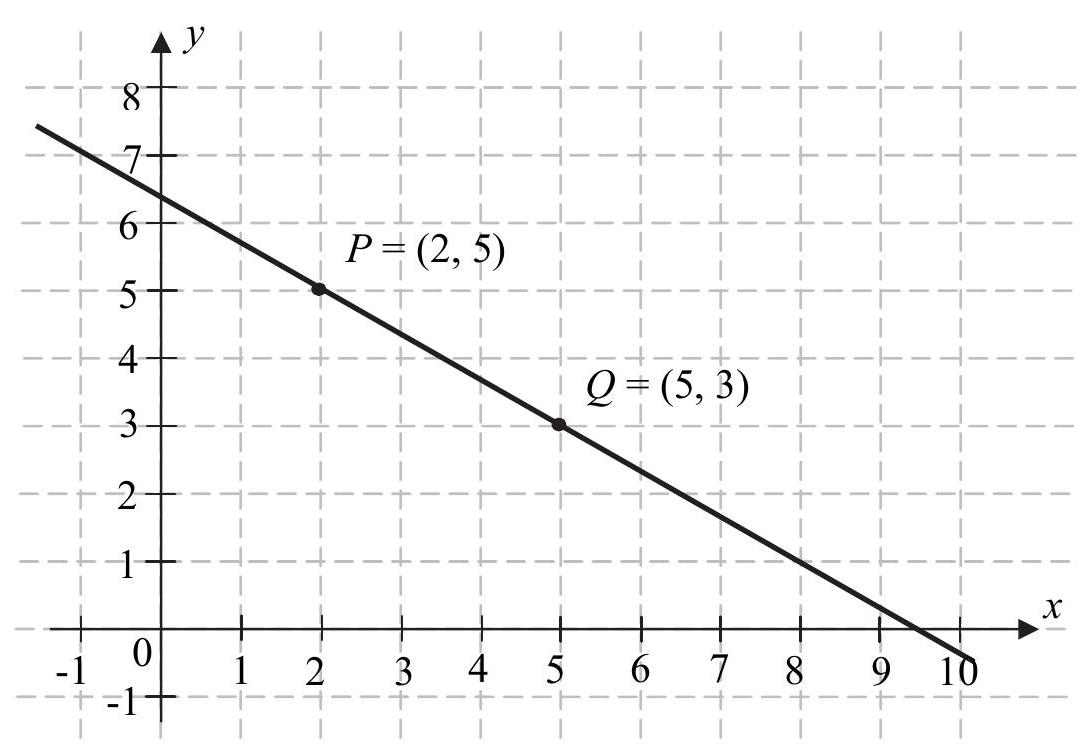
\includegraphics[max width=\textwidth, center]{2024_11_21_e19607c15353cb4d7e48g-04}

Współczynnik kierunkowy tej prostej jest równy\\
A. \(a=-\frac{3}{2}\)\\
B. \(a=-\frac{2}{3}\)\\
C. \(a=-\frac{2}{5}\)\\
D. \(a=-\frac{3}{5}\)

\section*{Zadanie 11. (1 pkt)}
W ciągu arytmetycznym \(\left(a_{n}\right)\) określonym dla \(n \geq 1\) dane są \(a_{1}=-4\) i \(r=2\). Którym wyrazem tego ciągu jest liczba 156 ?\\
A. 81 .\\
B. 80 .\\
C. 76 .\\
D. 77 .

\section*{Zadanie 12. (1 pkt)}
W rosnącym ciągu geometrycznym \(\left(a_{n}\right)\), określonym dla \(n \geq 1\), spełniony jest warunek \(a_{4}=3 a_{1}\). Iloraz \(q\) tego ciągu jest równy\\
A. \(q=\frac{1}{3}\)\\
B. \(q=\frac{1}{\sqrt[3]{3}}\)\\
C. \(q=\sqrt[3]{3}\)\\
D. \(q=3\)

BRUDNOPIS (nie podlega ocenie)\\

\includegraphics[max width=\textwidth, center]{2024_11_21_e19607c15353cb4d7e48g-05}

\section*{Zadanie 13. (1 pkt)}
Drabinę o długości 4 metrów oparto o pionowy mur, a jej podstawę umieszczono w odległości \(1,30 \mathrm{~m}\) od tego muru (zobacz rysunek).\\
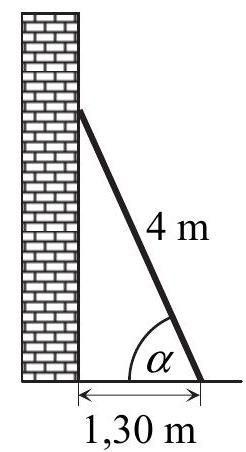
\includegraphics[max width=\textwidth, center]{2024_11_21_e19607c15353cb4d7e48g-06}

Kąt \(\alpha\), pod jakim ustawiono drabinę, spełnia warunek\\
A. \(0^{\circ}<\alpha<30^{\circ}\)\\
B. \(30^{\circ}<\alpha<45^{\circ}\)\\
C. \(45^{\circ}<\alpha<60^{\circ}\)\\
D. \(60^{\circ}<\alpha<90^{\circ}\)

\section*{Zadanie 14. (1 pkt)}
Kąt \(\alpha\) jest ostry i \(\sin \alpha=\frac{2}{5}\). Wówczas \(\cos \alpha\) jest równy\\
A. \(\frac{5}{2}\)\\
B. \(\frac{\sqrt{21}}{4}\)\\
C. \(\frac{3}{5}\)\\
D. \(\frac{\sqrt{21}}{5}\)

\section*{Zadanie 15. (1 pkt)}
W trójkącie równoramiennym \(A B C\) spełnione są warunki: \(|A C|=|B C|, \quad \Varangle C A B \mid=50^{\circ}\). Odcinek \(B D\) jest dwusieczną kąta \(A B C\), a odcinek \(B E\) jest wysokością opuszczoną z wierzchołka \(B\) na bok \(A C\). Miara kąta \(E B D\) jest równa\\
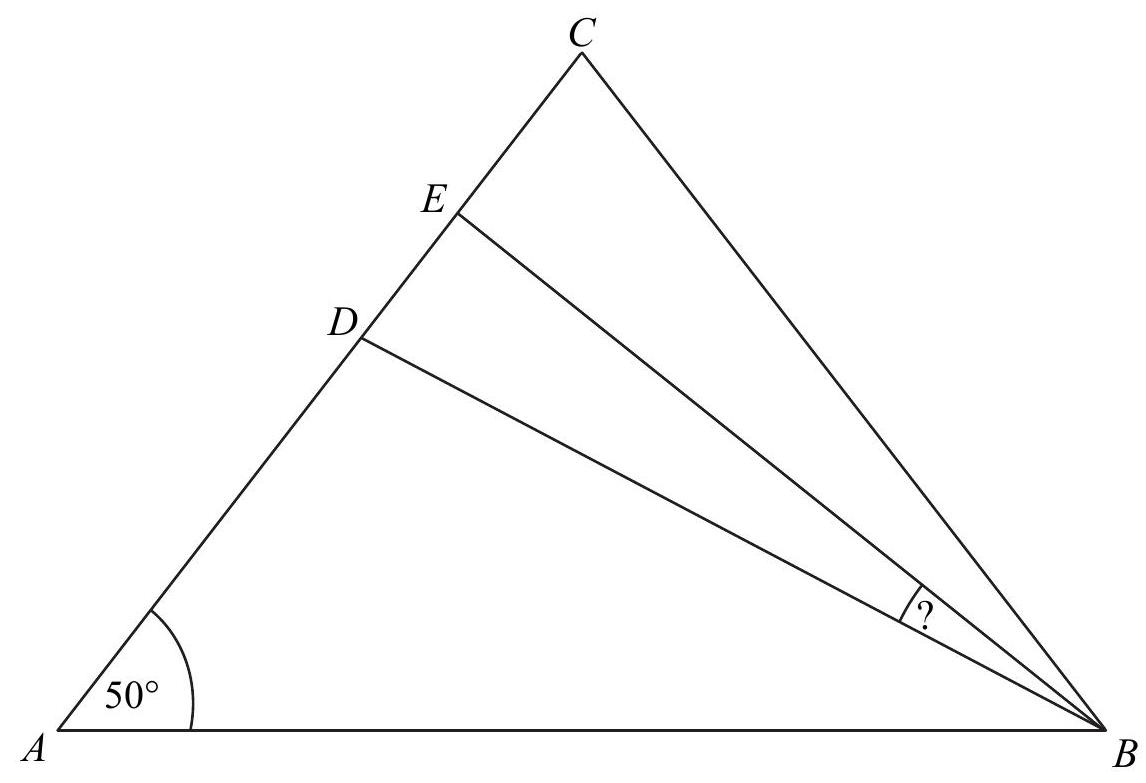
\includegraphics[max width=\textwidth, center]{2024_11_21_e19607c15353cb4d7e48g-06(1)}\\
A. \(10^{\circ}\)\\
B. \(12,5^{\circ}\)\\
C. \(13,5^{\circ}\)\\
D. \(15^{\circ}\)

BRUDNOPIS (nie podlega ocenie)\\

\includegraphics[max width=\textwidth, center]{2024_11_21_e19607c15353cb4d7e48g-07}

\section*{Zadanie 16. (1 pkt)}
Przedstawione na rysunku trójkąty są podobne.\\
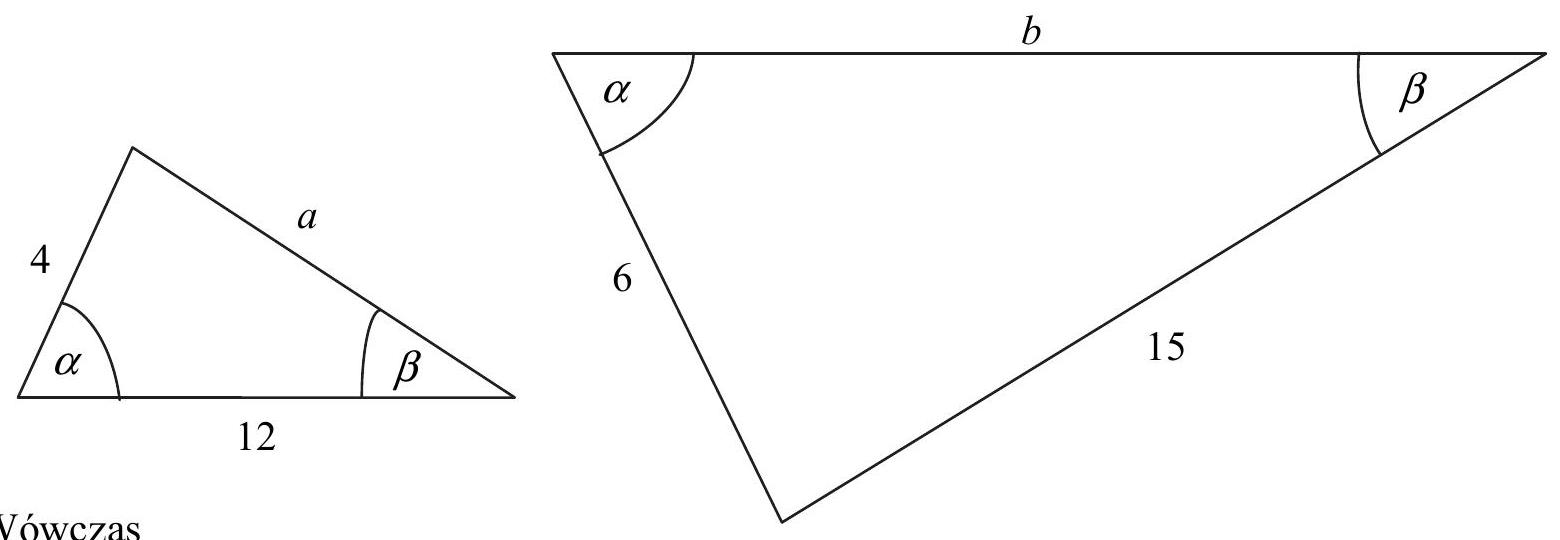
\includegraphics[max width=\textwidth, center]{2024_11_21_e19607c15353cb4d7e48g-08}

Wówczas\\
A. \(a=13, b=17\)\\
B. \(a=10, b=18\)\\
C. \(a=9, b=19\)\\
D. \(\quad a=11, b=13\)

\section*{Zadanie 17. (1 pkt)}
Proste o równaniach: \(y=2 m x-m^{2}-1\) oraz \(y=4 m^{2} x+m^{2}+1\) są prostopadłe dla\\
A. \(m=-\frac{1}{2}\)\\
B. \(m=\frac{1}{2}\)\\
C. \(m=1\)\\
D. \(m=2\)

\section*{Zadanie 18. (1 pkt)}
Dane są punkty \(M=(3,-5)\) oraz \(N=(-1,7)\). Prosta przechodząca przez te punkty ma równanie\\
A. \(y=-3 x+4\)\\
B. \(y=3 x-4\)\\
C. \(y=-\frac{1}{3} x+4\)\\
D. \(y=3 x+4\)

\section*{Zadanie 19. (1 pkt)}
Dane są punkty: \(P=(-2,-2), Q=(3,3)\). Odległość punktu \(P\) od punktu \(Q\) jest równa\\
A. 1\\
B. 5\\
C. \(5 \sqrt{2}\)\\
D. \(2 \sqrt{5}\)

\section*{Zadanie 20. (1 pkt)}
Punkt \(K=(-4,4)\) jest końcem odcinka \(K L\), punkt \(L\) leży na osi \(O x\), a środek \(S\) tego odcinka leży na osi \(O y\). Wynika stąd, że\\
A. \(S=(0,2)\)\\
B. \(S=(-2,0)\)\\
C. \(S=(4,0)\)\\
D. \(S=(0,4)\)

BRUDNOPIS (nie podlega ocenie)\\

\includegraphics[max width=\textwidth, center]{2024_11_21_e19607c15353cb4d7e48g-09}

\section*{Zadanie 21. (1 pkt)}
Okrąg przedstawiony na rysunku ma środek w punkcie \(O=(3,1)\) i przechodzi przez punkty \(S=(0,4)\) i \(T=(0,-2)\). Okrąg ten jest opisany przez równanie\\
A. \((x+3)^{2}+(y+1)^{2}=18\)\\
B. \((x-3)^{2}+(y+1)^{2}=18\)\\
C. \((x-3)^{2}+(y-1)^{2}=18\)\\
D. \((x+3)^{2}+(y-1)^{2}=18\)\\
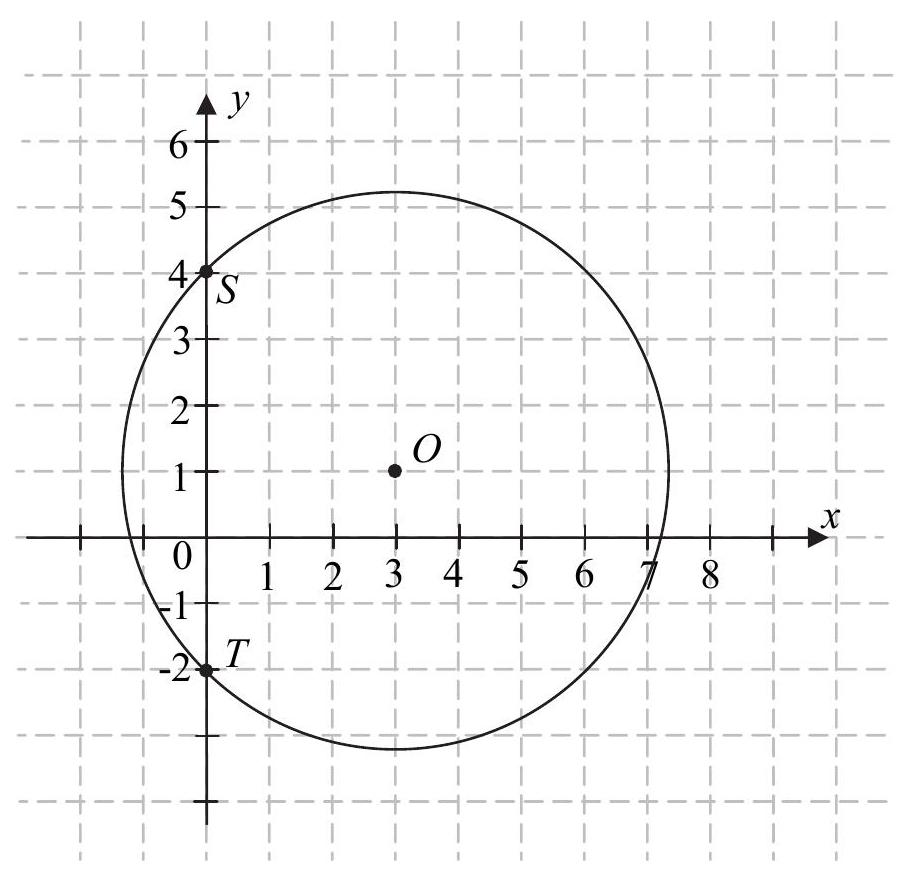
\includegraphics[max width=\textwidth, center]{2024_11_21_e19607c15353cb4d7e48g-10}

\section*{Zadanie 22. (1 pkt)}
Przekątna ściany sześcianu ma długość 2. Pole powierzchni całkowitej tego sześcianu jest równe\\
A. 24\\
B. \(12 \sqrt{2}\)\\
C. 12\\
D. \(16 \sqrt{2}\)

\section*{Zadanie 23. (1 pkt)}
Kula o promieniu 5 cm i stożek o promieniu podstawy 10 cm mają równe objętości. Wysokość stożka jest równa\\
A. \(\frac{25}{\pi} \mathrm{~cm}\)\\
B. 10 cm\\
C. \(\frac{10}{\pi} \mathrm{~cm}\)\\
D. 5 cm

\section*{Zadanie 24. (1 pkt)}
Średnia arytmetyczna zestawu danych:

\[
2,4,7,8,9
\]

jest taka sama jak średnia arytmetyczna zestawu danych:

\[
2,4,7,8,9, x
\]

Wynika stąd, że\\
A. \(x=0\)\\
B. \(x=3\)\\
C. \(x=5\)\\
D. \(x=6\)

\section*{Zadanie 25. (1 pkt)}
W pewnej klasie stosunek liczby dziewcząt do liczby chłopców jest równy 4:5. Losujemy jedną osobę z tej klasy. Prawdopodobieństwo tego, że będzie to dziewczyna, jest równe\\
A. \(\frac{4}{5}\)\\
B. \(\frac{4}{9}\)\\
C. \(\frac{1}{4}\)\\
D. \(\frac{1}{9}\)

BRUDNOPIS (nie podlega ocenie)\\

\includegraphics[max width=\textwidth, center]{2024_11_21_e19607c15353cb4d7e48g-11}

Zadanie 26. (2 pkt)\\
Wykaż, że dla każdej liczby rzeczywistej \(x\) i dla każdej liczby rzeczywistej \(y\) prawdziwa jest nierówność \(4 x^{2}-8 x y+5 y^{2} \geq 0\).

\begin{center}
\begin{tabular}{|c|c|c|c|c|c|c|c|c|c|c|c|c|c|c|c|c|c|c|c|c|c|}
\hline
 &  &  &  &  &  &  &  &  &  &  &  &  &  &  &  &  &  &  &  &  &  \\
\hline
 &  &  &  &  &  &  &  &  &  &  &  &  &  &  &  &  &  &  &  &  &  \\
\hline
 &  &  &  &  &  &  &  &  &  &  &  &  &  &  &  &  &  &  &  &  &  \\
\hline
 &  &  &  &  &  &  &  &  &  &  &  &  &  &  &  &  &  &  &  &  &  \\
\hline
 &  &  &  &  &  &  &  &  &  &  &  &  &  &  &  &  &  &  &  &  &  \\
\hline
 &  &  &  &  &  &  &  &  &  &  &  &  &  &  &  &  &  &  &  &  &  \\
\hline
 &  &  &  &  &  &  &  &  &  &  &  &  &  &  &  &  &  &  &  &  &  \\
\hline
 &  &  &  &  &  &  &  &  &  &  &  &  &  &  &  &  &  &  &  &  &  \\
\hline
 &  &  &  &  &  &  &  &  &  &  &  &  &  &  &  &  &  &  &  &  &  \\
\hline
 &  &  &  &  &  &  &  &  &  &  &  &  &  &  &  &  &  &  &  &  &  \\
\hline
 &  &  &  &  &  &  &  &  &  &  &  &  &  &  &  &  &  &  &  &  &  \\
\hline
 &  &  &  &  &  &  &  &  &  &  &  &  &  &  &  &  &  &  &  &  &  \\
\hline
 &  &  &  &  &  &  &  &  &  &  &  &  &  &  &  &  &  &  &  &  &  \\
\hline
 &  &  &  &  &  &  &  &  &  &  &  &  &  &  &  &  &  &  &  &  &  \\
\hline
 &  &  &  &  &  &  &  &  &  &  &  &  &  &  &  &  &  &  &  &  &  \\
\hline
 &  &  &  &  &  &  &  &  &  &  &  &  &  &  &  &  &  &  &  &  &  \\
\hline
 &  &  &  &  &  &  &  &  &  &  &  &  &  &  &  &  &  &  &  &  &  \\
\hline
 &  &  &  &  &  &  &  &  &  &  &  &  &  &  &  &  &  &  &  &  &  \\
\hline
 &  &  &  &  &  &  &  &  &  &  &  &  &  &  &  &  &  &  &  &  &  \\
\hline
 &  &  &  &  &  &  &  &  &  &  &  &  &  &  &  &  &  &  &  &  &  \\
\hline
 &  &  &  &  &  &  &  &  &  &  &  &  &  &  &  &  &  &  &  &  &  \\
\hline
 &  &  &  &  &  &  &  &  &  &  &  &  &  &  &  &  &  &  &  &  &  \\
\hline
 &  &  &  &  &  &  &  &  &  &  &  &  &  &  &  &  &  &  &  &  &  \\
\hline
 &  &  &  &  &  &  &  &  &  &  &  &  &  &  &  &  &  &  &  &  &  \\
\hline
 &  &  &  &  &  &  &  &  &  &  &  &  &  &  &  &  &  &  &  &  &  \\
\hline
 &  &  &  &  &  &  &  &  &  &  &  &  &  &  &  &  &  &  &  &  &  \\
\hline
 &  &  &  &  &  &  &  &  &  &  &  &  &  &  &  &  &  &  &  &  &  \\
\hline
 &  &  &  &  &  &  &  &  &  &  &  &  &  &  &  &  &  &  &  &  &  \\
\hline
 &  &  &  &  &  &  &  &  &  &  &  &  &  &  &  &  &  &  &  &  &  \\
\hline
 &  &  &  &  &  &  &  &  &  &  &  &  &  &  &  &  &  &  &  &  &  \\
\hline
 &  &  &  &  &  &  &  &  &  &  &  &  &  &  &  &  &  &  &  &  &  \\
\hline
 &  &  &  &  &  &  &  &  &  &  &  &  &  &  &  &  &  &  &  &  &  \\
\hline
 &  &  &  &  &  &  &  &  &  &  &  &  &  &  &  &  &  &  &  &  &  \\
\hline
 &  &  &  &  &  &  &  &  &  &  &  &  &  &  &  &  &  &  &  &  &  \\
\hline
 &  &  &  &  &  &  &  &  &  &  &  &  &  &  &  &  &  &  &  &  &  \\
\hline
 &  &  &  &  &  &  &  &  &  &  &  &  &  &  &  &  &  &  &  &  &  \\
\hline
 &  &  &  &  &  &  &  &  &  &  &  &  &  &  &  &  &  &  &  &  &  \\
\hline
 &  &  &  &  &  &  &  &  &  &  &  &  &  &  &  &  &  &  &  &  &  \\
\hline
 &  &  &  &  &  &  &  &  &  &  &  &  &  &  &  &  &  &  &  &  &  \\
\hline
 &  &  &  &  &  &  &  &  &  &  &  &  &  &  &  &  &  &  &  &  &  \\
\hline
 &  &  &  &  &  &  &  &  &  &  &  &  &  &  &  &  &  &  &  &  &  \\
\hline
 &  &  &  &  &  &  &  &  &  &  &  &  &  &  &  &  &  &  &  &  &  \\
\hline
 &  &  &  &  &  &  &  &  &  &  &  &  &  &  &  &  &  &  &  &  &  \\
\hline
 &  &  &  &  &  &  &  &  &  &  &  &  &  &  &  &  &  &  &  &  &  \\
\hline
 &  &  &  &  &  &  &  &  &  &  &  &  &  &  &  &  &  &  &  &  &  \\
\hline
\end{tabular}
\end{center}

\section*{Zadanie 27. (2 pkt)}
Rozwiąż nierówność \(2 x^{2}-4 x \geq x-2\).\\

\includegraphics[max width=\textwidth, center]{2024_11_21_e19607c15353cb4d7e48g-13}

Odpowiedź:

\begin{center}
\begin{tabular}{|c|l|c|c|}
\hline
\multirow{2}{*}{\begin{tabular}{c}
Wypelnia \\
egzaminator \\
\end{tabular}} & Nr zadania & 26. & 27. \\
\cline { 2 - 4 }
 & Maks. liczba pkt & 2 & \(\mathbf{2}\) \\
\cline { 2 - 4 }
 & Uzyskana liczba pkt &  &  \\
\hline
\end{tabular}
\end{center}

\section*{Zadanie 28. (2 pkt)}
Rozwiąż równanie \(4 x^{3}+4 x^{2}-x-1=0\).\\

\includegraphics[max width=\textwidth, center]{2024_11_21_e19607c15353cb4d7e48g-14}

Odpowiedź:

\section*{Zadanie 29. (2 pkt)}
Na rysunku przedstawiono wykres funkcji \(f\).\\
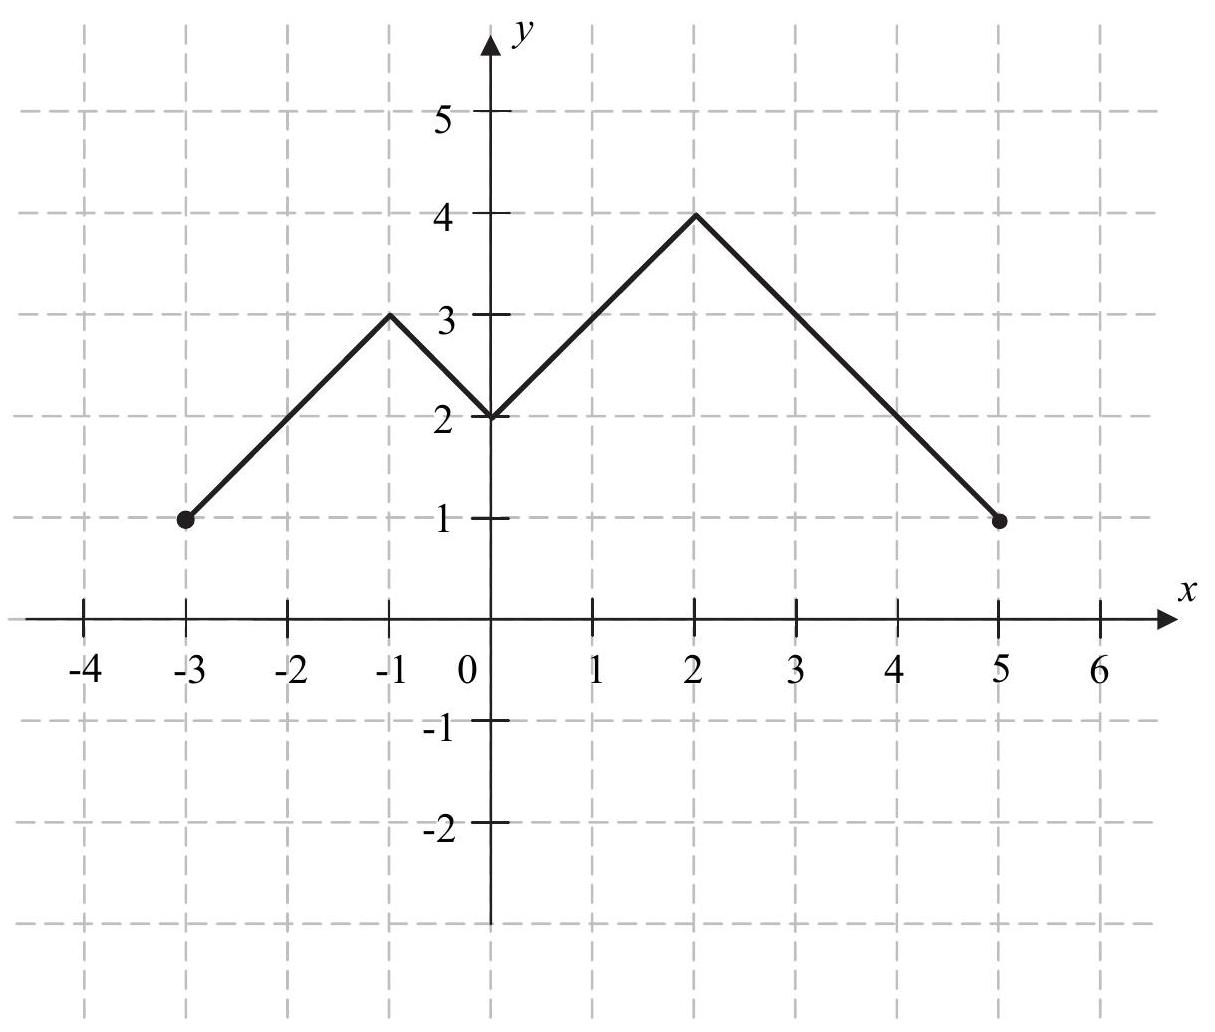
\includegraphics[max width=\textwidth, center]{2024_11_21_e19607c15353cb4d7e48g-15(1)}

Funkcja \(h\) określona jest dla \(x \in\langle-3,5\rangle\) wzorem \(h(x)=f(x)+q\), gdzie \(q\) jest pewną liczbą rzeczywistą. Wiemy, że jednym z miejsc zerowych funkcji \(h\) jest liczba \(x_{0}=-1\).\\
a) Wyznacz \(q\).\\
b) Podaj wszystkie pozostałe miejsca zerowe funkcji \(h\).

\begin{center}
\begin{tabular}{|c|c|c|c|c|c|c|c|c|c|c|c|c|c|c|c|c|c|c|c|c|c|c|c|c|c|c|c|c|c|c|c|c|}
\hline
 &  &  &  &  &  &  &  &  &  &  &  &  &  &  &  &  &  &  &  &  &  &  &  &  &  &  &  &  &  &  &  &  \\
\hline
 &  &  &  &  &  &  &  &  &  &  &  &  &  &  &  &  &  &  &  &  &  &  &  &  &  &  &  &  &  &  &  &  \\
\hline
 &  &  &  &  &  &  &  &  &  &  &  &  &  &  &  &  &  &  &  &  &  &  &  &  &  &  &  &  &  &  &  &  \\
\hline
 &  &  &  &  &  &  &  &  &  &  &  &  &  &  &  &  &  &  &  &  &  &  &  &  &  &  &  &  &  &  &  &  \\
\hline
 &  &  &  &  &  &  &  &  &  &  &  &  &  &  &  &  &  &  &  &  &  &  &  &  &  &  &  &  &  &  &  &  \\
\hline
 &  &  &  &  &  &  &  &  &  &  &  &  &  &  &  &  &  &  &  &  &  &  &  &  &  &  &  &  &  &  &  &  \\
\hline
 &  &  &  &  &  &  &  &  &  &  &  &  &  &  &  &  &  &  &  &  &  &  &  &  &  &  &  &  &  &  &  &  \\
\hline
 &  &  &  &  &  &  &  &  &  &  &  &  &  &  &  & 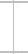
\includegraphics[max width=\textwidth]{2024_11_21_e19607c15353cb4d7e48g-15}
 &  &  &  &  &  &  &  &  &  &  &  &  &  &  &  &  \\
\hline
 &  &  &  &  &  &  &  &  &  &  &  &  &  &  &  &  &  &  &  &  &  &  &  &  &  &  &  &  &  &  &  &  \\
\hline
 &  &  &  &  &  &  &  &  &  &  &  &  &  &  &  &  &  &  &  &  &  &  &  &  &  &  &  &  &  &  &  &  \\
\hline
 &  &  &  &  &  &  &  &  &  &  &  &  &  &  &  &  &  &  &  &  &  &  &  &  &  &  &  &  &  &  &  &  \\
\hline
 &  &  &  &  &  &  &  &  &  &  &  &  &  &  &  &  &  &  &  &  &  &  &  &  &  &  &  &  &  &  &  &  \\
\hline
\end{tabular}
\end{center}

Odpowiedź: \(\qquad\)\\
\(\qquad\)

\begin{center}
\begin{tabular}{|c|l|c|c|}
\hline
\multirow{2}{*}{\begin{tabular}{c}
Wypetnia \\
egzaminator \\
\end{tabular}} & Nr zadania & 28. & 29. \\
\cline { 2 - 4 }
 & Maks. liczba pkt & 2 & 2 \\
\cline { 2 - 4 }
 & Uzyskana liczba pkt &  &  \\
\hline
\end{tabular}
\end{center}

Strona 15 z 24

\section*{Zadanie 30. (2 pkt)}
Dany jest skończony ciąg, w którym pierwszy wyraz jest równy 444, a ostatni jest równy 653 . Każdy wyraz tego ciągu, począwszy od drugiego, jest o 11 większy od wyrazu bezpośrednio go poprzedzającego. Oblicz sumę wszystkich wyrazów tego ciągu.\\

\includegraphics[max width=\textwidth, center]{2024_11_21_e19607c15353cb4d7e48g-16}

Odpowiedź:

\section*{Zadanie 31. (2 pkt)}
Dany jest okrąg o środku w punkcie \(O\). Prosta \(K L\) jest styczna do tego okręgu w punkcie \(L\), a środek \(O\) tego okręgu leży na odcinku \(K M\) (zob. rysunek). Udowodnij, że kąt \(K M L\) ma miarę \(31^{\circ}\).\\
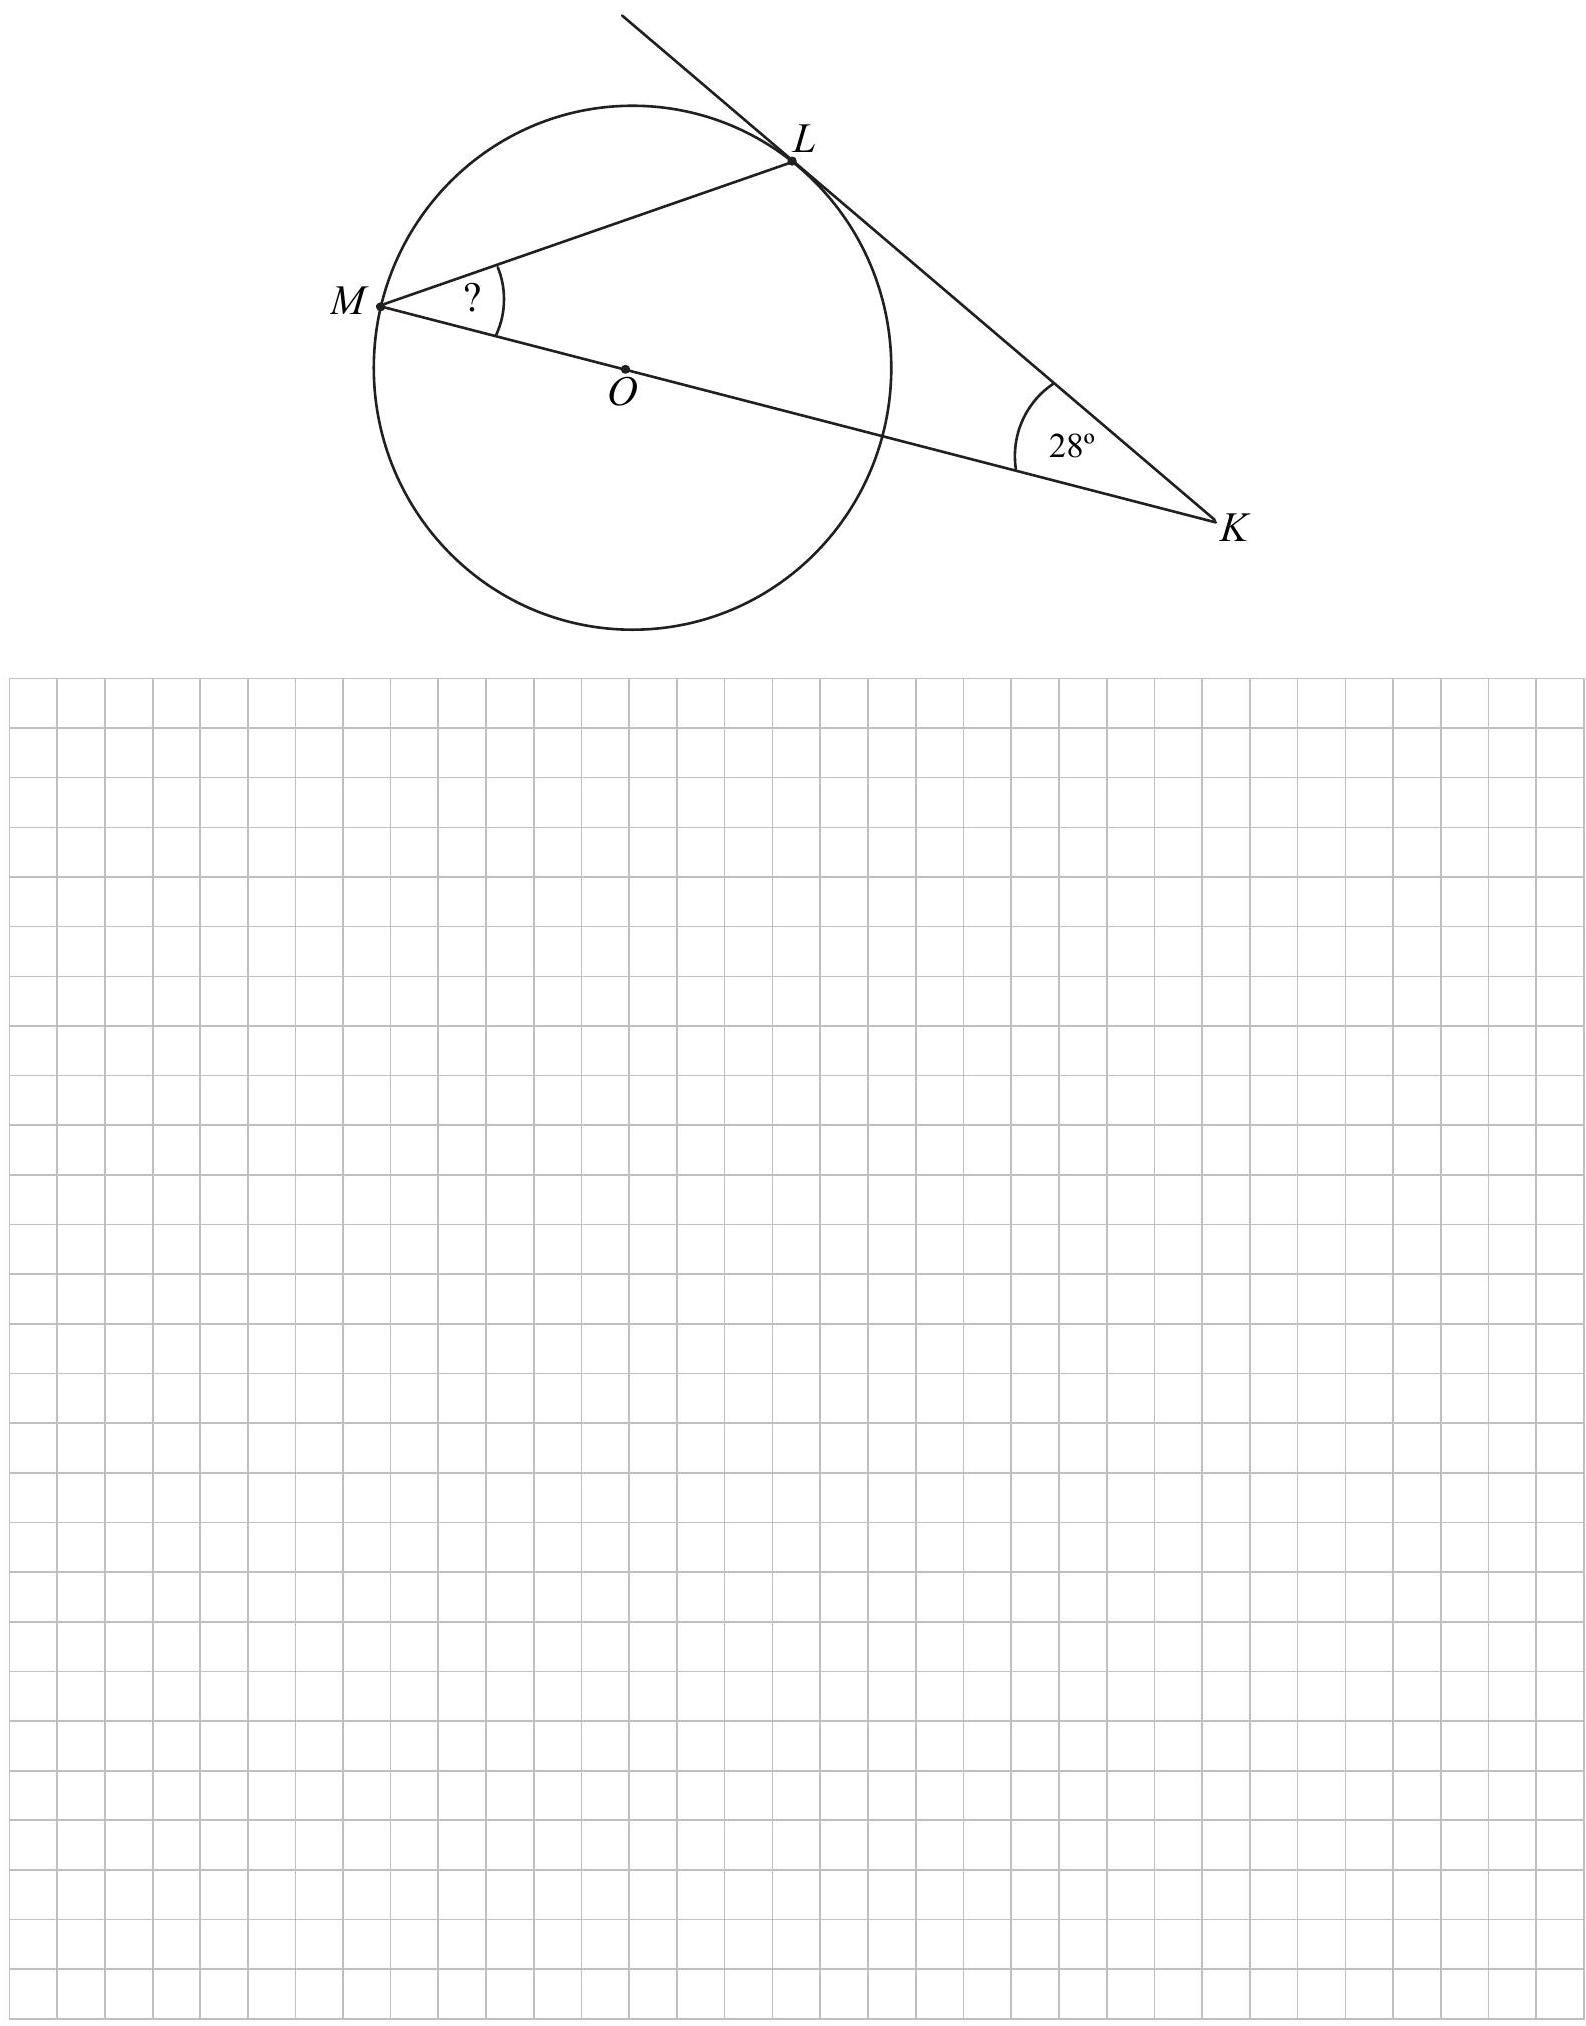
\includegraphics[max width=\textwidth, center]{2024_11_21_e19607c15353cb4d7e48g-17}

\begin{center}
\begin{tabular}{|c|l|c|c|}
\hline
\multirow{2}{*}{\begin{tabular}{c}
Wypelnia \\
egzaminator \\
\end{tabular}} & Nr zadania & \(\mathbf{3 0 .}\) & \(\mathbf{3 1 .}\) \\
\cline { 2 - 4 }
 & Maks. liczba pkt & \(\mathbf{2}\) & \(\mathbf{2}\) \\
\cline { 2 - 4 }
 & Uzyskana liczba pkt &  &  \\
\hline
\end{tabular}
\end{center}

\section*{Zadanie 32. (4 pkt)}
Wysokość graniastosłupa prawidłowego czworokątnego jest równa 16. Przekątna graniastosłupa jest nachylona do płaszczyzny jego podstawy pod kątem, którego cosinus jest równy \(\frac{3}{5}\). Oblicz pole powierzchni całkowitej tego graniastosłupa.\\

\includegraphics[max width=\textwidth, center]{2024_11_21_e19607c15353cb4d7e48g-18}\\

\includegraphics[max width=\textwidth, center]{2024_11_21_e19607c15353cb4d7e48g-19}

Odpowiedź:

\begin{center}
\begin{tabular}{|c|l|c|}
\hline
\multirow{2}{*}{\begin{tabular}{l}
Wypetnia \\
egzaminator \\
\end{tabular}} & Nr zadania & 32. \\
\cline { 2 - 3 }
 & Maks. liczba pkt & 4 \\
\cline { 2 - 3 }
 & Uzyskana liczba pkt &  \\
\hline
\end{tabular}
\end{center}

\section*{Zadanie 33. (4 pkt)}
Wśród 115 osób przeprowadzono badania ankietowe, związane z zakupami w pewnym kiosku. W poniższej tabeli przedstawiono informacje o tym, ile osób kupiło bilety tramwajowe ulgowe oraz ile osób kupiło bilety tramwajowe normalne.

\begin{center}
\begin{tabular}{|c|c|}
\hline
\begin{tabular}{c}
Rodzaj kupionych \\
biletów \\
\end{tabular} & Liczba osób \\
\hline
ulgowe & 76 \\
\hline
normalne & 41 \\
\hline
\end{tabular}
\end{center}

Uwaga! 27 osób spośród ankietowanych kupiło oba rodzaje biletów.\\
Oblicz prawdopodobieństwo zdarzenia polegającego na tym, że osoba losowo wybrana spośród ankietowanych nie kupiła żadnego biletu. Wynik przedstaw w formie nieskracalnego ułamka.

\begin{center}
\begin{tabular}{|c|c|c|c|c|c|c|c|c|c|c|c|c|c|c|c|c|c|c|c|c|c|c|c|}
\hline
 &  &  &  &  &  &  &  &  &  &  &  &  &  &  &  &  &  &  &  &  &  &  &  \\
\hline
 &  &  &  &  &  &  &  &  &  &  &  &  &  &  &  &  &  &  &  &  &  &  &  \\
\hline
 &  &  &  &  &  &  &  &  &  &  &  &  &  &  &  &  &  &  &  &  &  &  &  \\
\hline
 &  &  &  &  &  &  &  &  &  &  &  &  &  &  &  &  &  &  &  &  &  &  &  \\
\hline
 &  &  &  &  &  &  &  &  &  &  &  &  &  &  &  &  &  &  &  &  &  &  &  \\
\hline
 &  &  &  &  &  &  &  &  &  &  &  &  &  &  &  &  &  &  &  &  &  &  &  \\
\hline
 &  &  &  &  &  &  &  &  &  &  &  &  &  &  &  &  &  &  &  &  &  &  &  \\
\hline
 &  &  &  &  &  &  &  &  &  &  &  &  &  &  &  &  &  &  &  &  &  &  &  \\
\hline
 &  &  &  &  &  &  &  &  &  &  &  &  &  &  &  &  &  &  &  &  &  &  &  \\
\hline
 &  &  &  &  &  &  &  &  &  &  &  &  &  &  &  &  &  &  &  &  &  &  &  \\
\hline
 &  &  &  &  &  &  &  &  &  &  &  &  &  &  &  &  &  &  &  &  &  &  &  \\
\hline
 &  &  &  &  &  &  &  &  &  &  &  &  &  &  &  &  &  &  &  &  &  &  &  \\
\hline
 &  &  &  &  &  &  &  &  &  &  &  &  &  &  &  &  &  &  &  &  &  &  &  \\
\hline
 &  &  &  &  &  &  &  &  &  &  &  &  &  &  &  &  &  &  &  &  &  &  &  \\
\hline
 &  &  &  &  &  &  &  &  &  &  &  &  &  &  &  &  &  &  &  &  &  &  &  \\
\hline
 &  &  &  &  &  &  &  &  &  &  &  &  &  &  &  &  &  &  &  &  &  &  &  \\
\hline
 &  &  &  &  &  &  &  &  &  &  &  &  &  &  &  &  &  &  &  &  &  &  &  \\
\hline
 &  &  &  &  &  &  &  &  &  &  &  &  &  &  &  &  &  &  &  &  &  &  &  \\
\hline
 &  &  &  &  &  &  &  &  &  &  &  &  &  &  &  &  &  &  &  &  &  &  &  \\
\hline
 &  &  &  &  &  &  &  &  &  &  &  &  &  &  &  &  &  &  &  &  &  &  &  \\
\hline
 &  &  &  &  &  &  &  &  &  &  &  &  &  &  &  &  &  &  &  &  &  &  &  \\
\hline
 &  &  &  &  &  &  &  &  &  &  &  &  &  &  &  &  &  &  &  &  &  &  &  \\
\hline
 &  &  &  &  &  &  &  &  &  &  &  &  &  &  &  &  &  &  &  &  &  &  &  \\
\hline
 &  &  &  &  &  &  &  &  &  &  &  &  &  &  &  &  &  &  &  &  &  &  &  \\
\hline
 &  &  &  &  &  &  &  &  &  &  &  &  &  &  &  &  &  &  &  &  &  &  &  \\
\hline
 &  &  &  &  &  &  &  &  &  &  &  &  &  &  &  &  &  &  &  &  &  &  &  \\
\hline
 &  &  &  &  &  &  &  &  &  &  &  &  &  &  &  &  &  &  &  &  &  &  &  \\
\hline
 &  &  &  &  &  &  &  &  &  &  &  &  &  &  &  &  &  &  &  &  &  &  &  \\
\hline
 &  &  &  &  &  &  &  &  &  &  &  &  &  &  &  &  &  &  &  &  &  &  &  \\
\hline
 &  &  &  &  &  &  &  &  &  &  &  &  &  &  &  &  &  &  &  &  &  &  &  \\
\hline
 &  &  &  &  &  &  &  &  &  &  &  &  &  &  &  &  &  &  &  &  &  &  &  \\
\hline
 &  &  &  &  &  &  &  &  &  &  &  &  &  &  &  &  &  &  &  &  &  &  &  \\
\hline
 &  &  &  &  &  &  &  &  &  &  &  &  &  &  &  &  &  &  &  &  &  &  &  \\
\hline
 &  &  &  &  &  &  &  &  &  &  &  &  &  &  &  &  &  &  &  &  &  &  &  \\
\hline
 &  &  &  &  &  &  &  &  &  &  &  &  &  &  &  &  &  &  &  &  &  &  &  \\
\hline
 &  &  &  &  &  &  &  &  &  &  &  &  &  &  &  &  &  &  &  &  &  &  &  \\
\hline
\end{tabular}
\end{center}

\begin{center}

\includegraphics[max width=\textwidth]{2024_11_21_e19607c15353cb4d7e48g-21}
\end{center}

Odpowiedź:

\begin{center}
\begin{tabular}{|c|l|c|}
\hline
\multirow{2}{*}{\begin{tabular}{l}
Wypełnia \\
egzaminator \\
\end{tabular}} & Nr zadania & 33. \\
\cline { 2 - 3 }
 & Maks. liczba pkt & 4 \\
\cline { 2 - 3 }
 & Uzyskana liczba pkt &  \\
\hline
\end{tabular}
\end{center}

\section*{Zadanie 34. (5 pkt)}
Biegacz narciarski Borys wyruszył na trasę biegu o 10 minut później niż inny zawodnik, Adam. Metę zawodów, po przebyciu 15-kilometrowej trasy biegu, obaj zawodnicy pokonali równocześnie. Okazało się, że wartość średniej prędkości na całej trasie w przypadku Borysa była o \(4,5 \frac{\mathrm{~km}}{\mathrm{~h}}\) większa niż w przypadku Adama. Oblicz, w jakim czasie Adam pokonał całą trasę biegu.

\begin{center}
\begin{tabular}{|c|c|c|c|c|c|c|c|c|c|c|c|c|c|c|c|c|c|c|c|c|c|}
\hline
 &  &  &  &  &  &  &  &  &  &  &  &  &  &  &  &  &  &  &  &  &  \\
\hline
 &  &  &  &  &  &  &  &  &  &  &  &  &  &  &  &  &  &  &  &  &  \\
\hline
 &  &  &  &  &  &  &  &  &  &  &  &  &  &  &  &  &  &  &  &  &  \\
\hline
 &  &  &  &  &  &  &  &  &  &  &  &  &  &  &  &  &  &  &  &  &  \\
\hline
 &  &  &  &  &  &  &  &  &  &  &  &  &  &  &  &  &  &  &  &  &  \\
\hline
 &  &  &  &  &  &  &  &  &  &  &  &  &  &  &  &  &  &  &  &  &  \\
\hline
 &  &  &  &  &  &  &  &  &  &  &  &  &  &  &  &  &  &  &  &  &  \\
\hline
 &  &  &  &  &  &  &  &  &  &  &  &  &  &  &  &  &  &  &  &  &  \\
\hline
 &  &  &  &  &  &  &  &  &  &  &  &  &  &  &  &  &  &  &  &  &  \\
\hline
 &  &  &  &  &  &  &  &  &  &  &  &  &  &  &  &  &  &  &  &  &  \\
\hline
 &  &  &  &  &  &  &  &  &  &  &  &  &  &  &  &  &  &  &  &  &  \\
\hline
 &  &  &  &  &  &  &  &  &  &  &  &  &  &  &  &  &  &  &  &  &  \\
\hline
 &  &  &  &  &  &  &  &  &  &  &  &  &  &  &  &  &  &  &  &  &  \\
\hline
 &  &  &  &  &  &  &  &  &  &  &  &  &  &  &  &  &  &  &  &  &  \\
\hline
 &  &  &  &  &  &  &  &  &  &  &  &  &  &  &  &  &  &  &  &  &  \\
\hline
 &  &  &  &  &  &  &  &  &  &  &  &  &  &  &  &  &  &  &  &  &  \\
\hline
 &  &  &  &  &  &  &  &  &  &  &  &  &  &  &  &  &  &  &  &  &  \\
\hline
 &  &  &  &  &  &  &  &  &  &  &  &  &  &  &  &  &  &  &  &  &  \\
\hline
 &  &  &  &  &  &  &  &  &  &  &  &  &  &  &  &  &  &  &  &  &  \\
\hline
 &  &  &  &  &  &  &  &  &  &  &  &  &  &  &  &  &  &  &  &  &  \\
\hline
 &  &  &  &  &  &  &  &  &  &  &  &  &  &  &  &  &  &  &  &  &  \\
\hline
 &  &  &  &  &  &  &  &  &  &  &  &  &  &  &  &  &  &  &  &  &  \\
\hline
 &  &  &  &  &  &  &  &  &  &  &  &  &  &  &  &  &  &  &  &  &  \\
\hline
 &  &  &  &  &  &  &  &  &  &  &  &  &  &  &  &  &  &  &  &  &  \\
\hline
 &  &  &  &  &  &  &  &  &  &  &  &  &  &  &  &  &  &  &  &  &  \\
\hline
 &  &  &  &  &  &  &  &  &  &  &  &  &  &  &  &  &  &  &  &  &  \\
\hline
 &  &  &  &  &  &  &  &  &  &  &  &  &  &  &  &  &  &  &  &  &  \\
\hline
 &  &  &  &  &  &  &  &  &  &  &  &  &  &  &  &  &  &  &  &  &  \\
\hline
 &  &  &  &  &  &  &  &  &  &  &  &  &  &  &  &  &  &  &  &  &  \\
\hline
 &  &  &  &  &  &  &  &  &  &  &  &  &  &  &  &  &  &  &  &  &  \\
\hline
 &  &  &  &  &  &  &  &  &  &  &  &  &  &  &  &  &  &  &  &  &  \\
\hline
 &  &  &  &  &  &  &  &  &  &  &  &  &  &  &  &  &  &  &  &  &  \\
\hline
 &  &  &  &  &  &  &  &  &  &  &  &  &  &  &  &  &  &  &  &  &  \\
\hline
 &  &  &  &  &  &  &  &  &  &  &  &  &  &  &  &  &  &  &  &  &  \\
\hline
 &  &  &  &  &  &  &  &  &  &  &  &  &  &  &  &  &  &  &  &  &  \\
\hline
 &  &  &  &  &  &  &  &  &  &  &  &  &  &  &  &  &  &  &  &  &  \\
\hline
 &  &  &  &  &  &  &  &  &  &  &  &  &  &  &  &  &  &  &  &  &  \\
\hline
 &  &  &  &  &  &  &  &  &  &  &  &  &  &  &  &  &  &  &  &  &  \\
\hline
 &  &  &  &  &  &  &  &  &  &  &  &  &  &  &  &  &  &  &  &  &  \\
\hline
 &  &  &  &  &  &  &  &  &  &  &  &  &  &  &  &  &  &  &  &  &  \\
\hline
 &  &  &  &  &  &  &  &  &  &  &  &  &  &  &  &  &  &  &  &  &  \\
\hline
 &  &  &  &  &  &  &  &  &  &  &  &  &  &  &  &  &  &  &  &  &  \\
\hline
\end{tabular}
\end{center}

\begin{center}

\includegraphics[max width=\textwidth]{2024_11_21_e19607c15353cb4d7e48g-23}
\end{center}

Odpowiedź:

\begin{center}
\begin{tabular}{|c|l|c|}
\hline
\multirow{2}{*}{\begin{tabular}{l}
Wypelnia \\
egzaminator \\
\end{tabular}} & Nr zadania & 34. \\
\cline { 2 - 3 }
 & Maks. liczba pkt & 5 \\
\cline { 2 - 3 }
 & Uzyskana liczba pkt &  \\
\hline
\end{tabular}
\end{center}

\section*{BRUDNOPIS (nie podlega ocenie)}

\end{document}